\section{Calculs approchés d'intégrales}

% \todoinline{Je pense que le cas "par morceaux" est pénible à montrer et peu utile. Se limiter à continue me semble suffisant.}

\begin{theo}{\textsc{Riemann}}
    \marginnote[0cm]{\cite{acamanes}}
    Pour tout entier naturel $n$ non nul, la \emph{somme de \textsc{Riemann}} associée à $f$ sur le segment $[a, b]$ est 
    $$S_n \defeq \frac{b-a}{n} \sum\limits_{k=0}^{n-1} f \left( a + k \frac{b-a}{n} \right).$$
    Si $f$ est continue sur $[a, b]$, alors, 
    $$\lim_{n \to + \infty} S_n = \int_a^b f(t) \d t.$$
\end{theo}

%\begin{marginfigure}[-3cm]
%    %https://tex.stackexchange.com/questions/476702/riemann-sum-approaches-area-under-curve

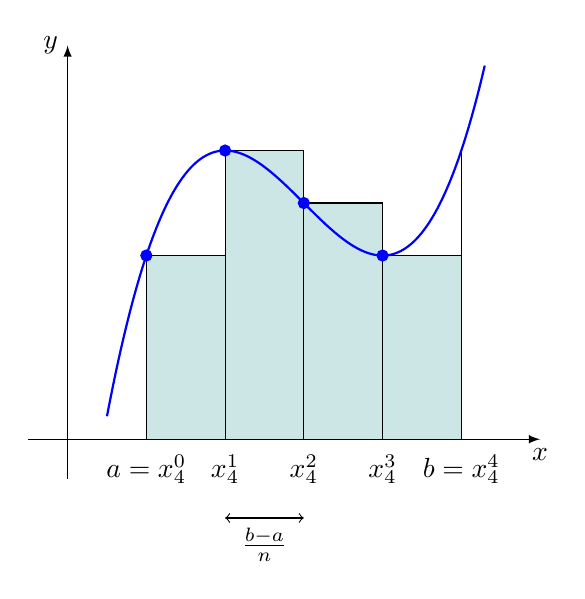
\begin{tikzpicture}[scale=1,declare function={f(\x)=((1/3)*(\x)^(3)-3*(\x)^(2)+8*\x-3;}]
\coordinate (start) at (.8,{f(.8)});
\coordinate (x0) at (1,{f(1)});
\coordinate (x1) at (2,{f(2)});
\coordinate (x2) at (3,{f(3)});
\coordinate (x3) at (4,{f(4)});
\coordinate (x4) at (5,{f(5)});
\coordinate (end) at (5.05,{f(5.05)});
\draw[fill=teal!20!white] (1,0) rectangle (2,{f(1)});
\draw[fill=teal!20!white] (2,0) rectangle (3,{f(2)});
\draw[fill=teal!20!white] (3,0) rectangle (4,{f(3)});
\draw[fill=teal!20!white] (4,0) rectangle (5,{f(4)});
\draw (5,0)--(5,{f(5)});
\draw [-latex] (-0.5,0) -- (6,0) node (xaxis) [below] {$x$};
\draw [-latex] (0,-0.5) -- (0,5) node [left] {$y$};
\foreach \x/\xtext in {1/a=x^0_{4} ,2/x^1_{4}, 3/x^2_{4} , 4/x^3_{4} , 5/b=x^4_{4}}
 \draw[xshift=\x cm] (0pt,3pt) -- (0pt,0pt) 
node[below=2pt,fill=white,font=\normalsize]
  {$\xtext$};
\draw[domain=.5:5.3,samples=200,variable=\x,blue,thick] plot ({\x},{f(\x)});                 
\foreach \n in {0,1,2,3}
\draw[blue,fill=blue] (x\n) circle (2pt) node[font=\normalsize] {$ $};    
\draw[<->] (2,-1)--(3,-1) node[below,midway] {$\frac{b-a}{n}$};      
\end{tikzpicture}
%\end{marginfigure}

\begin{preuve}
    
\end{preuve}

\todoinline{Je mettrais plutôt un thème sur les calculs approchés d'intégrales : rectangles gauche, médian, trapèze, Simpson ?}

\todoarmand{Comptez-vous reprendre comme tels les exercices que vous avez mis dans le dossier documents ?}

\todoinline{On peut prendre ce qu'on veut dans les documents, il n'y a pas de copyright. Je n'ai aucune idée. De mémoire il y a un joli dessin pour la méthode des trapèzes. Ce qui est important (à mes yeux) c'est qu'on a à chaque fois, et de manière optimale, la rapidité de la convergence.}

\todoarmand{J'écris tout le contenu du document, ça nous donne une base.}

Dans tout le problème, $a$ et $b$ désignent deux réels tels que $a < b$. Pour tout entier naturel $p$ non nul, on note $(x_i)_{i\in\llbracket 0, p \rrbracket}$ la subdivision régulière de $[a, b]$ de pas $\frac{b-a}{p}$. Ainsi, pour tout $i \in \llbracket 0, p \rrbracket$,
\[
x_i = a + i \frac{b-a}{p}.
\]
Une méthode d'intégration est d'\emph{ordre} au moins $n$ si elle est exacte sur les polynômes de degrés inférieurs ou égaux $n$ et non exacte pour au moins un polynôme de degré $n+1$.

\subsection{Méthode des rectangles à gauche}

La méthode composée des rectangles à gauche consiste à découper le segment $[a, b]$ en $p$ sous-segments puis à appliquer la méthode simple des rectangles à gauche sur chacune de ces subdivisions :
% \begin{columns}{2}
\[
I_p^g(f) = \frac{b-a}{p} \sum_{i=0}^{p-1} f(x_i).
\]
%
% \columnbreak
%
% \begin{center}
%   \scalebox{0.3}{\input{chapitres/integration/documents/figures/approx_rect_g.pdf_t}}
% \end{center}
% \end{columns}

Dans toute cette partie, $f$ désigne une fonction de classe $\mathscr{C}^1$ sur le segment $[a, b]$. On note $F$ une primitive de $f$ et $M_1 = \sup_{[a,b]} \module{f'}$.

\begin{enumerate}
    \item Montrer que, pour tout $i \in \llbracket 0, p-1 \rrbracket$,
\[
\module{F(x_{i+1}) - F(x_i) - (x_{i+1} - x_i) F'(x_i)} \leq \frac{M_1}{2} (x_{i+1}-x_i)^2.
\]

    \item En déduire que
\[
\module{\int_{[a,b]} f - I_p^g(f)} \leq \frac{M_1 (b-a)^2}{2 p}.
\]

    \item Montrer que cette borne est atteinte pour $f : x \mapsto x - a$.

    \item Montrer que la méthode des rectangles à gauche est d'ordre $0$.
\end{enumerate}

\subsection{Méthode des rectangles médians}

La méthode composée des rectangles médians consiste à découper le segment $[a, b]$ en $p$ sous-segments puis à appliquer la méthode simple des rectangles médians sur chacune de ces subdivisions :
% \begin{columns}{2}
\[
I_p^m(f) = \frac{b-a}{p} \sum_{i=0}^{p-1} f\left(\frac{x_i + x_{i+1}}{2} \right).
\]
%
% \columnbreak
%
% \begin{center}
% \scalebox{0.3}{\input{chapitres/integration/documents/figures/approx_rect_m.pdf_t}}
% \end{center}
% \end{columns}

Dans toute cette partie, $f$ désigne une fonction de classe $\mathscr{C}^2$ sur le segment $[a, b]$. On note $F$ une primitive de $f$ et $M_2 = \sup_{[a,b]} \module{f''}$. Pour tout entier $i \in \interent{0}{p-1}$, on pose $\gamma_i = \frac{x_i + x_{i+1}}{2}$

\begin{enumerate}
\item Soit $i \in \interent{0}{p-1}$.
\begin{enumerate}
    \item Montrer que
    \[
    (x_{i+1} - x_i) f(\gamma_i) = \int_{x_i}^{x_{i+1}} \left(f(\gamma_i) + (t - \gamma_i) f'(\gamma_i) \right) \d t.
    \]
    
    \item En déduire que
    \[
    \module{F(x_{i+1}) - F(x_i) - (x_{i+1} - x_i) F'(\gamma_i)}
    \leq \frac{M_2}{24} (x_{i+1} - x_i)^3.
    \]
\end{enumerate}

\item Montrer que
\[
\module{\int_{[a,b]} f - I_p^m(f)} \leq \frac{M_2 (b-a)^3}{24 p^2}
\]

\item Montrer que cette borne est atteinte pour $f : x \mapsto (x - a)^2$.

\item Montrer que la méthode des rectangles médians est d'ordre $1$.

\end{enumerate}

\subsection{Méthode des trapèzes}

La méthode composée des trapèzes consiste à découper le segment $[a, b]$ en $p$ sous-segments puis à appliquer la méthode simple des trapèzes sur chacune de ces subdivisions :
%\begin{colonnes}{2}
\[
I_p^t(f) =  \frac{b-a}{p} \sum_{i=0}^{p-1} \frac{f(x_i) + f(x_{i+1})}{2}.
\]
%
%\columnbreak
%
%\begin{center}
%\scalebox{0.3}{\input{figures/approx_trap.pdf_t}}
%\end{center}
%\end{colonnes}

On suppose dans cette partie que $f$ est une fonction de classe $\mathscr{C}^2$ et on note $M_2 = \sup_{[a,b]} \module{f''}$. Pour tout $i \in \interent{0}{p-1}$, on note $\phi_i$ l'approximation affine sur $[x_i, x_{i+1}]$ de $f$ et $g_i = f - \phi_i$.

\begin{enumerate}
\item À l'aide d'intégrations par parties, montrer que, pour tout $i \in \interent{0}{p-1}$,
\[
\int_{x_i}^{x_{i+1}} f''(t) (t - x_i) (x_{i+1} - t) \d t = - 2 \int_{x_i}^{x_{i+1}} g_i(t) \d t.
\]

\item En déduire que
\[
\module{\int_{[a,b]} f - I_p^t(f)} \leq \frac{M_2 (b-a)^3}{12 p^2}.
\]

\item Montrer que cette borne est atteinte pour $f : x \mapsto (x - a)^2$.

\item Montrer que la méthode des trapèzes est d'ordre $1$.

\item Montrer que, lorsque $f'' \geq 0$ (en particulier lorsque $f$ est convexe), pour tout entier naturel $p$, $\int_{[a,b]} f \leq I_p^t(f)$.

\end{enumerate}

\subsection{Méthode de \textsc{Simpson}}

La méthode composée de Simpson consiste à découper le segment $[a, b]$ en $p$ sous-segments puis à approcher, sur chacune de ces subdivisions, la fonction $f$ par un polynôme de degré inférieur ou égal à $2$ :
\[
I_p^s(f) = \frac{b-a}{6 p} \sum_{i=0}^{p-1} \left[f(x_i)+ 4 f\left(\frac{x_i + x_{i+1}}{2}\right) + f(x_{i+1})\right].
\]
\begin{enumerate}
\item Soit $g \in \mathscr{C}^5([a, b], \R)$ une fonction impaire. On note $K_5 = \sup_{[a,b]} \module{g^{(5)}}$. En utilisant la formule de \mathsc{Taylor} avec reste intégral pour $g$ et $g'$, montrer que
\[
\module{g(x) - \frac{x}{3} (g'(x) + 2 g'(0))} \leq \frac{K_5}{180} \module{x}^5.
\]

On suppose dans cette partie que $f$ est une fonction de classe $\mathscr{C}^4$ sur le segment $[a, b]$. On pose $M_4 = \sup_{[a,b]} \module{f^{(4)}}$.

\item Montrer que, pour tout $i \in \interent{0}{p-1}$,
\[
\module{F(x_{i+1}) - F(x_i) - \frac{1}{6p} \left[ f(x_{i+1}) + f(x_i) + 4 f\left(\frac{x_{i+1}+x_i}{2}\right) \right]}
\leq
\frac{M_4 (x_{i+1} - x_i)^5}{2880}.
\]

\emph{Poser $g : t \mapsto F\left(\frac{x_{i+1}+x_i}{2}+t\right) - F\left(\frac{x_{i+1}+x_i}{2}-t\right)$.}

\item En déduire que
\[
\module{I_p^s(f) - \int_a^b f(t) \d t} \leq \frac{M_4 (b-a)^5}{2880 p^4}.
\]
\end{enumerate}
On peut montrer que la méthode de Simpson est d'ordre $3$. On peut augmenter le nombre des n\oe{}uds où est évaluée la fonction à intégrer ($2$ n\oe{}uds pour la méthode des trapèzes, $3$ pour la méthode de Simpson,\ldots). Ces méthodes sont appelées \emph{méthodes de \textsc{Newton}--\textsc{Cotes}}. Cependant, lorsque le nombre de n\oe{}uds dépasse $8$, des coefficients négatifs apparaissent ce qui engendre des erreurs d'arrondis. \\

Les sommes de \textsc{Riemann} permettent de calculer des intégrales mais leur convergence est lente comme le montre l'exercice suivant.

\begin{exercice}
    \marginnote[0cm]{Source : \cite{maths-france} Planche no 37. Intégration sur un segment}
    Soit $f$ une fonction de classe $\mathscr{C}^2$ sur $[0, 1]$. Déterminer le réel $a$ tel que:
    $$\int_0^1 f(t) \d t - \frac{1}{n} \sum_{k=1}^{n-1} f \left( \frac{k}{n} \right) =\lim\limits_{n \to + \infty} \frac{a}{n} + o \left( \frac{1}{n} \right).$$
    \end{exercice}